% !Mode:: "TeX:UTF-8"

\documentclass{beamer}
\usetheme{uestcthesis}
\begin{document}
\begin{frame}
\title{分布式在线程序评测系统——web端实现}
\author{\begin{tabular}{r@{ }l} 
答辩人      & 李昀 \\
专业 & 通信工程\\
学号 & 2010013100008\\
指导老师 & 饶力\\
\end{tabular}}
\titlepage
\end{frame}

\begin{frame}
\frametitle{Outline}
\tableofcontents[pausesections]
\end{frame}

\section{课题研究背景及意义}
\subsection{课题背景}
\begin{frame}{课题背景}{黑盒测试}
\begin{itemize}
	\item 测试者只知道程序的输入、输出和系统的功能
	\item 按照一定的规范设计出一系列测试案例来进行测试
\end{itemize}
\pause
\begin{exampleblock}{$A+B$问题:输入两个数字$a$和$b$,返回它们的和$a+b$}
\begin{itemize}
	\item 规范输入输出格式
	\item 构建测试用例:如输入$1 2 $,期望输出$3$
	\item 对于给定的程序依次使用构建的测试用例来进行测试
\end{itemize}
\end{exampleblock}
\end{frame}

\begin{frame}{课题背景}{黑盒测试}
\begin{alertblock}{手动测试}
\begin{itemize}
	\item 速度慢
	\item 效率低
	\item 不适合大规模作业
\end{itemize}
\end{alertblock}
\pause
\begin{block}{自动测试}
\begin{itemize}
	\item 速度快
	\item 高效率
	\item 在线测试
\end{itemize}
\end{block}
\end{frame}

\subsection{课题意义}
\begin{frame}{课题意义}{课题应用}
\begin{itemize}
	\item 程序设计竞赛

	本系统将被应用在即将到来的第12届电子科技大学程序设计校赛
	\item 计算机程序语言教学

	本系统已经被用在数学学院C语言上机练习教学中
\end{itemize}
\end{frame}

\section{系统实现}
\subsection{系统架构}
\begin{frame}{系统实现}{系统架构}
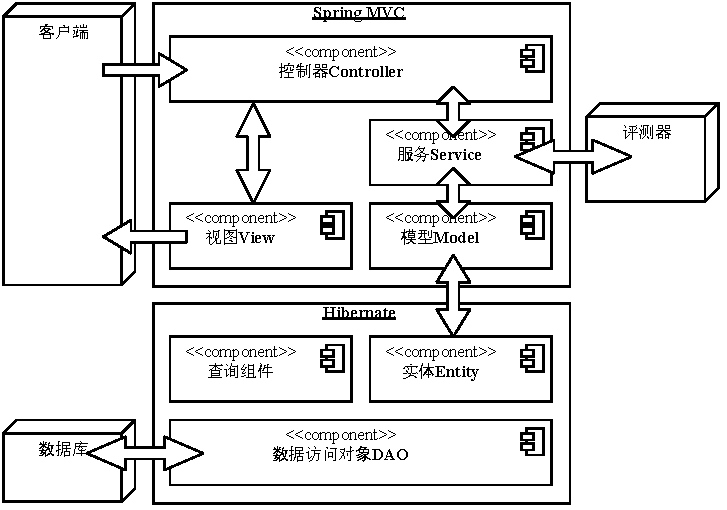
\includegraphics[width=0.9\textwidth]{pics/Architecture.pdf}
\end{frame}

\begin{frame}{系统实现}{系统架构}
\begin{itemize}
	\item 控制器Controller- 负责转发请求,对请求进行处理。
	\item 视图View - 图形界面设计。
	\item 模型Model和服务Service - 编写程序应有的功能(实现算法等等)、进行数据管理和数据库设计。
\end{itemize}
\end{frame}

%\begin{frame}{系统实现}{设计过程}
%\begin{itemize}
%	\item 需求驱动开发
%	\item 首先决定用户需要的功能
%	\item 构建用户界面
%	\item 确定后台控制器功能
%	\item 确定需要的服务和数据
%	\item 确定数据库模型
%\end{itemize}
%\end{frame}
\subsection{数据库模块}
\begin{frame}{系统实现}{数据库模块}
\begin{itemize}
	\item HQL查询语言

非常强大的查询语言,有意识的被设计为完全面向对象的查询,它可以理解如继承、多态 和关联之类的概念。

	\item DTO

用于保存数据库查询结果。

	\item Condition

确定数据库查询范围。

	\item DAO

执行数据库查询。
\end{itemize}
\end{frame}

\begin{frame}{系统实现}{数据库模块}
\begin{itemize}
	\item HQL = Select (DTO) From (数据库) Where (Condition)
	\item DTO = DAO.execute(HQL)
\end{itemize}
\pause
\begin{alertblock}{为什么要这样设计?}
避免手动构造查询语句(费时费力,难以维护)
\end{alertblock}
\pause
\begin{alertblock}{实现方式}
\begin{itemize}
	\item 反射(Reflection)
	\item 注解(Annotation)
\end{itemize}
\end{alertblock}
\end{frame}

\begin{frame}{系统实现}{数据库模块}
\begin{itemize}
	\item DTO通过注解来声明查询的字段
	\item Condition通过注解来声明限制条件以及限制字段
	\item 通过反射机制将注解装换成HQL语言
\end{itemize}
\end{frame}

\begin{frame}[containsverbatim]{系统实现}{数据库模块}
\begin{verbatim}
@Fields({"userId", "userName"})
public class UserListDTO {...}

public class UserCondition {
  @Exp(type = ConditionType.LIKE)
  public String userName;
}

Select userId, userName From User 
  Where userName like '%userName%'
\end{verbatim}
\end{frame}

\subsection{控制器与服务}
\begin{frame}{系统实现}{控制器与服务}
\begin{itemize}
	\item 控制器负责逻辑功能
	\item 服务实现各种算法
	\item 服务调用数据库模块完成数据库操作
\end{itemize}
\pause
\begin{exampleblock}{例:登陆功能}
控制器得到用户输入的账户和密码后,调用服务得到对应的用户实体。然后判断密码是否正确,如果正确就将该实体保存到用户会话中,否则返回密码错误信息。

控制器不直接操作数据库,服务也不参与密码验证。
\end{exampleblock}
\end{frame}

\begin{frame}{系统实现}{权限控制}
\begin{itemize}
	\item 链接权限
	\begin{itemize}
		\item 有些地址需要特殊的登录权限,例如题目编辑页面只有管理员才能访问
		\item 通过注解来声明某个控制器需要的权限
		\item 通过AOP在每次控制器运行前进行权限验证
	\end{itemize}
	\item 操作权限
	\begin{itemize}
		\item 有些操作需要特殊的权限,例如用户只允许修改自己的信息
		\item 在控制器代码中完成
	\end{itemize}
\end{itemize}
\end{frame}

\begin{frame}{系统实现}{Judge Service}
%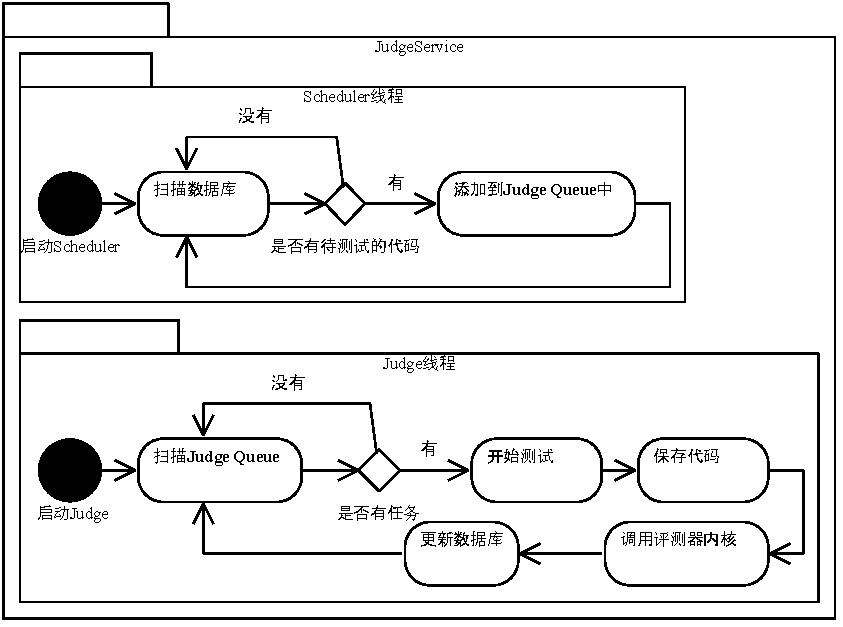
\includegraphics[width=0.9\textwidth]{pics/JudgeActivity.pdf}
\begin{itemize}
	\item 轮询评测列表中的待测代码
	\item 设置环境参数,调用评测器内核对代码进行黑盒测试
	\item 得到结果后更新
\end{itemize}
\end{frame}

\subsection{前端}
\begin{frame}{系统实现}{前端}
\begin{itemize}
	\item 单页应用
	\begin{itemize}
		\item 节约带宽
		\item 将视图部分交给客户器来执行
	\end{itemize}
	\item AngularJS
	\begin{itemize}
		\item 完善的路由功能
		\item 对文档的操作是基于声明的,而不是基于命令(与JQuery的区别)
		\item 完整的MVC支持,可以实现很多功能(动态加载、自动同步等)
	\end{itemize}
\end{itemize}
\end{frame}

%\begin{frame}{系统实现}{一次完整的交互过程}
%\begin{enumerate}
%	\item 用户打开Login in菜单,并在里面填入自己的用户名和密码
%	\item 在用户填入用户名和密码的同时,由于AngularJS的双向绑定效果,对应的变量也发生改变
%	\item 用户单击登陆按钮
%	\item 绑定在按钮上的事件开始执行,首先对密码进行加密,然后通过/user/login这个地址将登陆信息POST给服务器
%	\item 接收到响应后根据返回的结果来判断是否登陆成功,然后通知给用户
%\end{enumerate}
%\end{frame}

\begin{frame}{系统实现}{特点}
\begin{itemize}
	\item 前端简洁,一目了然
	\item 格式统一,表达能力强
	\begin{itemize}
		\item 采用markdown语言来格式化文本
		\item 支持LATEX格式的数学公式
	\end{itemize}
	\item 拥有完善的管理界面
\end{itemize}
\end{frame}

\section{系统测试}
\subsection{集成测试}
\begin{frame}{系统测试}{集成测试}
\begin{itemize}
	\item 单元测试
	\item 集成测试
	\item 模拟浏览器行为
	\item 将用户的所有可能的操作都模拟一次,以确保整个系统各个功能均无异常
	\item 直接通过mockMVC框架来模仿浏览器操作,与真实环境一模一样
\end{itemize}
\end{frame}
\subsection{压力测试}
\begin{frame}{系统测试}{压力测试}
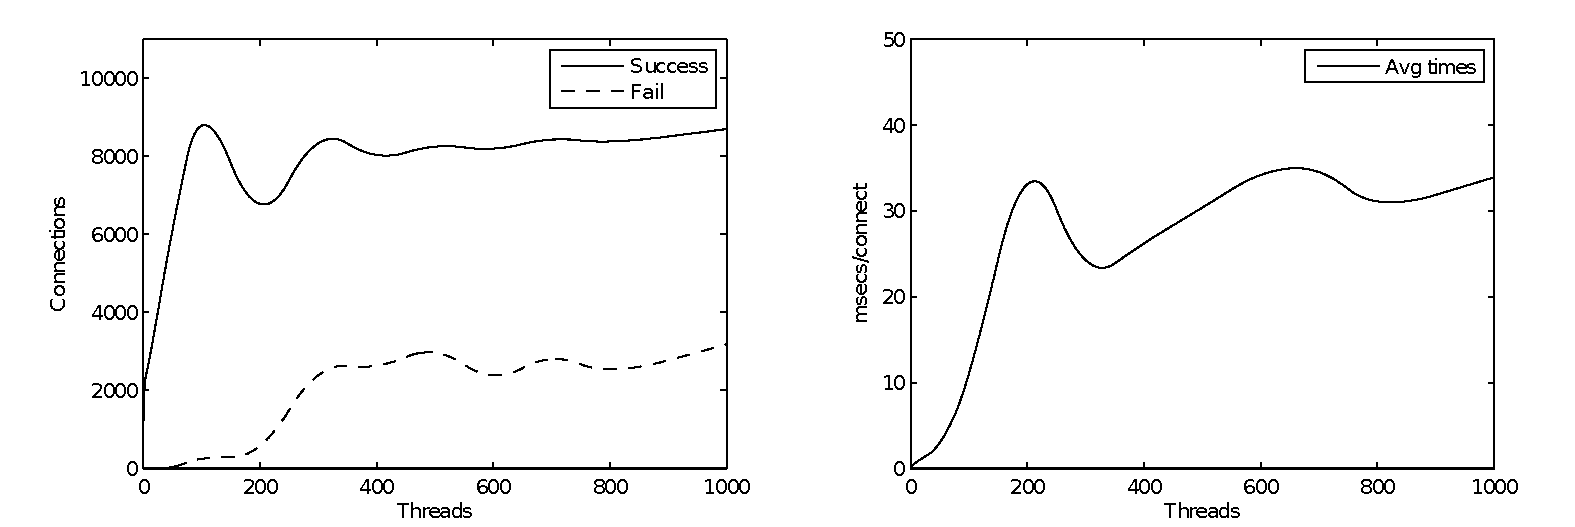
\includegraphics[width=0.9\textwidth]{pics/indexTest.pdf}

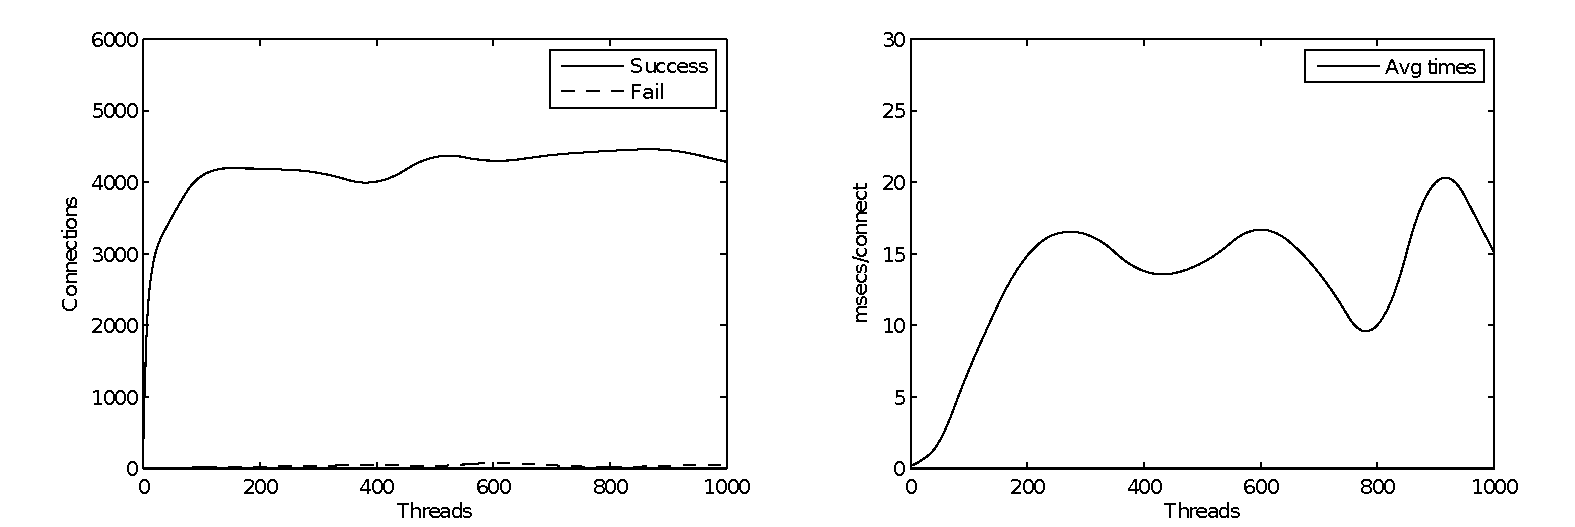
\includegraphics[width=0.9\textwidth]{pics/rankListTest.pdf}
\end{frame}

\section{总结}
\begin{frame}{总结}
从系统上线到现在,目前本系统已经有481位注册用户,211题不同的题目,2010次评测记录,举办过一次训练赛,这期间没有发生任何数据丢失、系统崩溃的事件,充分说明了本系统良好的结构以及完善的测试。
\end{frame}
\begin{frame}{致谢}
感谢学院和各位老师在百忙之中给了我这次提前答辩的机会,感谢我的指导老师饶力为我毕设开题到答辩提供的帮助,谢谢!
\end{frame}
\end{document} 